\documentclass{article}
\usepackage[paperwidth=4.2in,paperheight=4.2in,margin=0.1in]{geometry}
\usepackage{tikz}
\usetikzlibrary{shapes,arrows.meta,positioning}
\definecolor{boxblue}{RGB}{45,90,150}
\definecolor{boxorange}{RGB}{210,110,30}
\definecolor{armgdt}{RGB}{140,80,220}
\definecolor{warnred}{RGB}{220,60,60}
\pagestyle{empty}
\begin{document}
\begin{center}
\vspace*{\fill}
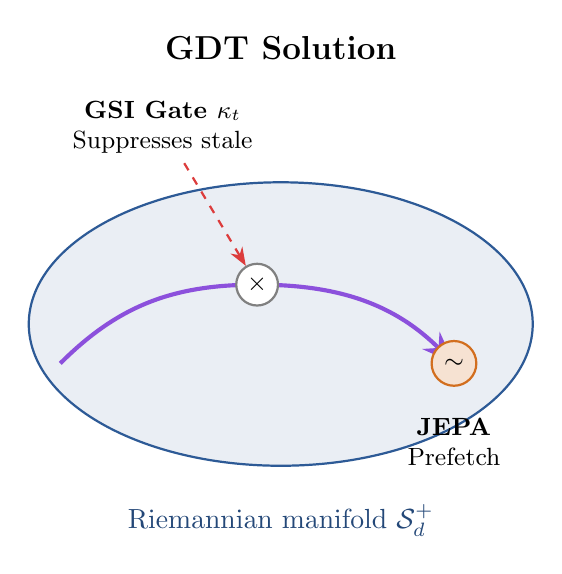
\begin{tikzpicture}[font=\sffamily]
% Title
\node[font=\large\bfseries] at (0, 3.5) {GDT Solution};

% Manifold
\draw[thick, fill=boxblue!10, draw=boxblue] (0, 0) ellipse (3.2cm and 1.8cm);

% Trajectory
\draw[line width=1.5pt, armgdt, -{Stealth[scale=1.2]}] (-2.8, -0.5) to[out=45, in=180] (-0.3, 0.5) to[out=0, in=135] (2.2, -0.5);

% Gate
\node[circle, fill=white, draw=gray, thick, inner sep=2pt, font=\small] (gate) at (-0.3, 0.5) {$\times$};
\node[align=center, font=\small] (gatelabel) at (-1.5, 2.5) {\textbf{GSI Gate $\kappa_t$}\\Suppresses stale};
\draw[thick, dashed, warnred, -{Stealth[scale=1.0]}] (gatelabel) -- (gate);

% JEPA
\node[circle, fill=boxorange!20, draw=boxorange, thick, inner sep=3pt, font=\small] (jepa) at (2.2, -0.5) {$\sim$};
\node[align=center, font=\small] at (2.2, -1.5) {\textbf{JEPA}\\Prefetch};

% Manifold Label
\node[font=\normalsize, text=boxblue!80!black] at (0, -2.5) {Riemannian manifold $\mathcal{S}_d^+$};
\end{tikzpicture}
\vspace*{\fill}
\end{center}
\end{document}
